% !TeX root = ../MQF_Manuale_Master.tex
% Capitoli/MQF_Cap_15_Programmazione_Stocastica_II.tex

\chapter{Soluzione e valore dell'informazione}

\label{cap:soluzione-valore-informazione}

\medskip

Il Capitolo~\ref{cap:programmazione-stocastica-due-stadi} ha costruito un
programma stocastico lineare a due stadi. La decisione iniziale $x$ viene
assunta prima di conoscere quale scenario si realizzer\`a; dopo
l'osservazione dell'incertezza, una decisione di ricorso $y_s$ permette di
adattare il piano alle condizioni dello scenario $s$.

Con un insieme finito di scenari, il problema \`e stato scritto nella forma

\[
\max_{x\in\mathcal X}
\left\{
c'x+
\sum_{s\in\mathcal S}p_sQ_s(x)
\right\},
\]

dove $Q_s(x)$ rappresenta il valore ottimo del problema di secondo stadio
nello scenario $s$.

La formulazione individua quale problema debba essere risolto, ma lascia
aperte alcune domande essenziali. Non ogni decisione iniziale garantisce
necessariamente l'esistenza di una risposta ammissibile in tutti gli scenari.
Il valore del ricorso cambia al variare di $x$ e questa dipendenza
contribuisce a determinare la soluzione ottima. Inoltre, la decisione ottenuta
tenendo conto dell'intera distribuzione degli scenari pu\`o essere confrontata
con decisioni costruite utilizzando informazioni differenti.

Il presente capitolo passa quindi dalla \emph{costruzione del modello} alla
\emph{lettura della sua soluzione}.

\medskip

\noindent
\textbf{Domanda guida:} quali propriet\`a deve possedere una decisione
stocastica, come si determina il compromesso tra scenari diversi e quanto
vale disporre di una migliore informazione sul futuro?

\medskip

Il primo problema riguarda la fattibilit\`a del ricorso. Una decisione di
primo stadio pu\`o risultare conveniente sotto il profilo economico ma
generare, in uno o pi\`u scenari, un problema di secondo stadio privo di
soluzioni ammissibili. Occorre quindi distinguere il valore del ricorso
dalla stessa possibilit\`a di effettuare una correzione dopo la realizzazione
dell'incertezza.

Il secondo problema riguarda la dipendenza della funzione di ricorso dalla
decisione iniziale. Nel caso lineare, tale funzione presenta una struttura
che pu\`o essere analizzata e interpretata: modificare $x$ cambia le risorse
con cui il decisore affronta gli scenari futuri e, di conseguenza, modifica
anche il valore delle migliori azioni correttive disponibili.

Questi elementi conducono alla soluzione del programma stocastico, che
indicheremo con

\[
x^{SP}
\]

e al corrispondente valore ottimo

\[
z^{SP}.
\]

La soluzione stocastica non identifica la decisione migliore per uno scenario
particolare. Essa individua una decisione iniziale unica, assunta prima della
rivelazione dell'incertezza, che tiene conto congiuntamente delle conseguenze
prodotte nei diversi scenari e delle rispettive probabilit\`a.

Nel caso guida SVB--ALM, $x^{SP}$ rappresenta quindi una composizione iniziale
dell'attivo comune a tutte le possibili evoluzioni future. La gestione della
liquidit\`a e del funding pu\`o invece adattarsi allo scenario attraverso i
vettori di ricorso $y_s$. Il problema consiste nel comprendere quale
allocazione iniziale produca il miglior equilibrio tra redditivit\`a corrente
e capacit\`a di affrontare condizioni future differenti.

Il valore di questa impostazione pu\`o essere compreso soltanto attraverso
opportuni termini di confronto. Considereremo per questo una decisione
costruita sostituendo i dati incerti con valori medi e, all'estremo opposto,
una situazione ideale nella quale lo scenario futuro sia conosciuto prima
della decisione iniziale. I confronti tra questi problemi permetteranno di
misurare sia il valore della soluzione stocastica sia il valore
dell'informazione perfetta.

Il capitolo compir\`a inoltre un ulteriore passaggio. Nel modello a due stadi
l'intera incertezza rilevante viene rivelata tra la decisione iniziale e il ricorso. Nei problemi finanziari l'informazione pu\`o invece arrivare
progressivamente. Introdurremo dapprima un modello a tre stadi, nel quale una
prima decisione correttiva viene assunta sulla base di informazione ancora
parziale, e utilizzeremo questa struttura per mostrare come la
non anticipativit\`a dipenda dalla storia effettivamente osservata.

Il caso a tre stadi consentir\`a infine di riconoscere la struttura generale
dei problemi multistadio, nei quali nodi informativi, decisioni contingenti e
storia osservata sostituiscono la semplice separazione tra un primo e un
secondo stadio.

La parte conclusiva del capitolo torner\`a alla struttura computazionale del
problema. La forma estesa introdotta nel Capitolo 14 presenta blocchi di
vincoli scenario-specifici collegati dalla decisione iniziale comune. Questa
struttura permette di comprendere perch\`e, una volta fissato $x$, i problemi
di ricorso possano essere trattati separatamente e introduce il principio
alla base dei metodi di decomposizione.

\medskip

\noindent
\textbf{Obiettivi della lezione.}

Al termine del capitolo lo studente dovr\`a essere in grado di:

\begin{itemize}

\item analizzare la fattibilit\`a e le principali propriet\`a della funzione
di ricorso in un programma stocastico lineare;

\item interpretare la soluzione stocastica come compromesso tra decisione
iniziale comune e risposte scenario-specifiche;

\item costruire e confrontare soluzione stocastica, Expected Value e
wait-and-see, interpretando EVPI e VSS;

\item comprendere il passaggio dal modello a due stadi a problemi con
informazione progressiva, riconoscendo il ruolo della non anticipativit\`a
nei modelli a tre e pi\`u stadi;

\item riconoscere la struttura per scenari del problema e il principio di
separabilit\`a che motiva i metodi di decomposizione.

\end{itemize}

\section{Fattibilit\`a del ricorso}

\label{sec:cap15-fattibilita-ricorso}

Nel programma stocastico a due stadi introdotto nel
Capitolo~\ref{cap:programmazione-stocastica-due-stadi}, una decisione iniziale
$x$ viene valutata tenendo conto delle migliori decisioni di ricorso
disponibili nei diversi scenari.

Prima di studiare il valore della funzione di ricorso occorre tuttavia
verificare una questione pi\`u fondamentale: dopo avere scelto $x$ e osservato
lo scenario, esiste effettivamente almeno una decisione di secondo stadio che
soddisfa tutti i vincoli?

Per lo scenario $s$, il problema di secondo stadio \`e stato scritto nella
forma

\[
Q_s(x)
=
\max_{y_s\in\mathcal X_s}
\left\{
q_s'y_s:
T_sx+W_sy_s=h_s
\right\}.
\]

La funzione $Q_s(x)$ descrive il valore della migliore risposta disponibile
nello scenario $s$, ma tale valore pu\`o essere determinato soltanto se
l'insieme delle decisioni di secondo stadio ammissibili non \`e vuoto.

\begin{definition}[Ricorso ammissibile]

Fissati una decisione di primo stadio $x\in\mathcal X$ e uno scenario
$s\in\mathcal S$, il ricorso \`e \emph{ammissibile} se esiste almeno una
decisione

\[
y_s\in\mathcal X_s
\]

tale che

\[
T_sx+W_sy_s=h_s.
\]

\end{definition}

La condizione riguarda esclusivamente la fattibilit\`a del secondo stadio,
non ancora il suo valore economico. Due decisioni iniziali possono entrambe
ammettere una risposta di ricorso nello stesso scenario e produrre valori di
$Q_s(x)$ molto diversi.

Viceversa, una decisione $x$ pu\`o appartenere all'insieme ammissibile del
primo stadio e tuttavia generare, in uno degli scenari, un problema di secondo
stadio privo di soluzioni ammissibili.

Questa osservazione conduce a due propriet\`a della struttura di ricorso che
\`e utile distinguere.

\begin{definition}[Ricorso completo]

Il problema di secondo stadio possiede \emph{ricorso completo} se la
struttura di ricorso consente di rendere ammissibile il secondo stadio per
ogni possibile vettore del termine noto del sistema.

Nella relazione

\[
W_sy_s=h_s-T_sx,
\]

la propriet\`a richiede quindi che, qualunque sia il vettore posto a destra
dell'uguaglianza, esista almeno una decisione di ricorso ammissibile capace
di soddisfare il sistema.

\end{definition}

Si tratta di una propriet\`a forte. Essa non considera soltanto i termini noti
che possono essere prodotti dalle decisioni e dagli scenari effettivamente
contenuti nel modello, ma richiede che la tecnologia di ricorso sia in grado
di compensare qualsiasi termine noto del sistema di secondo stadio.

Una nozione meno restrittiva, e spesso pi\`u rilevante nelle applicazioni,
\`e la seguente.

\begin{definition}[Ricorso relativamente completo]

Un programma stocastico a due stadi possiede \emph{ricorso relativamente completo} se, per ogni decisione di primo stadio ammissibile

\[
x\in\mathcal X
\]

e per ogni scenario

\[
s\in\mathcal S,
\]

esiste almeno una decisione di ricorso

\[
y_s\in\mathcal X_s
\]

tale che

\[
T_sx+W_sy_s=h_s.
\]

\end{definition}

La differenza tra le due nozioni riguarda dunque l'insieme dei termini noti
per i quali si richiede la fattibilit\`a del secondo stadio.

Il ricorso completo richiede che la struttura di ricorso possa soddisfare
qualsiasi possibile termine noto del sistema. Il ricorso relativamente completo
richiede invece la fattibilit\`a soltanto per i termini noti effettivamente
generati dalle decisioni

\[
x\in\mathcal X
\]

e dagli scenari considerati nel modello.

La seconda propriet\`a \`e quindi relativa alla struttura complessiva del
problema: modificando l'insieme delle decisioni ammissibili di primo stadio
oppure l'insieme degli scenari, pu\`o cambiare anche la validit\`a del
ricorso relativamente completo.

Le due nozioni possono essere sintetizzate come segue.

\begin{center}
\begin{tabular}{p{4.3cm}p{10.0cm}}
\hline
\textbf{Propriet\`a} & \textbf{Significato} \\
\hline
\emph{Ricorso completo}
&
Il secondo stadio \`e ammissibile per qualsiasi possibile termine noto che
debba essere compensato dalla struttura di ricorso.
\\[4pt]

\emph{Ricorso relativamente completo}
&
Il secondo stadio \`e ammissibile per tutti i termini noti effettivamente
generati dalle decisioni $x\in\mathcal X$ e dagli scenari del modello.
\\
\hline
\end{tabular}
\end{center}

Il ricorso completo \`e pertanto una propriet\`a pi\`u forte del ricorso relativamente  completo. Un modello pu\`o possedere ricorso relativamente completo
anche quando la propria capacit\`a di correzione non sarebbe sufficiente a
fronteggiare termini noti arbitrariamente sfavorevoli.

Nel caso ALM questa distinzione assume un significato immediato. La banca pu\`o
utilizzare strumenti di riequilibrio, come la raccolta di nuovo funding, ma
tali strumenti sono soggetti a limiti di capacit\`a. Non \`e quindi realistico
supporre che qualsiasi deficit di liquidit\`a possa essere compensato. La
questione rilevante \`e piuttosto verificare se tutte le decisioni iniziali
considerate ammissibili lascino alla banca una capacit\`a di correzione
sufficiente in ciascuno degli scenari previsti.

\subsection{Un esempio con capacit\`a limitata di funding}

Consideriamo un problema ridotto con due classi di attivo e risorse iniziali

\[
A_0=10.
\]

Indichiamo con $x$ l'ammontare investito nella classe di attivo pi\`u liquida.
La composizione iniziale \`e pertanto

\[
\begin{pmatrix}
x\\
10-x
\end{pmatrix},
\qquad
0\leq x\leq10.
\]

Alla data di ricorso deve essere soddisfatto un fabbisogno di liquidit\`a

\[
d=8.
\]

Consideriamo due scenari. Nello scenario ordinario, i coefficienti che
trasformano le due posizioni iniziali in liquidit\`a disponibile sono

\[
a_1'
=
(1,\;0.6),
\]

mentre nello scenario avverso sono

\[
a_2'
=
(1,\;0.2).
\]

La prima classe mantiene quindi la propria capacit\`a di generare liquidit\`a,
mentre la seconda diventa molto meno efficace nello scenario avverso.

Dopo l'osservazione dello scenario la banca pu\`o utilizzare nuovo funding
$u_s$ e mantenere un'eventuale giacenza residua $g_s$, con

\[
g_s\geq0,
\qquad
0\leq u_s\leq\bar u_s.
\]

Le capacit\`a massime di funding sono

\[
\bar u_1=1,
\qquad
\bar u_2=2.
\]

Il bilancio di secondo stadio \`e

\[
a_s'
\begin{pmatrix}
x\\
10-x
\end{pmatrix}
+
u_s
=
8+g_s.
\]

Poich\`e $g_s\geq0$, il funding minimo necessario nello scenario $s$ coincide
con il deficit di liquidit\`a quando tale deficit \`e positivo.

Nello scenario ordinario la liquidit\`a generata dagli attivi \`e

\[
x+0.6(10-x)
=
6+0.4x.
\]

Il funding minimo richiesto \`e quindi

\[
u_1^{\min}(x)
=
\max\{0,\;2-0.4x\}.
\]

Il ricorso \`e ammissibile se

\[
u_1^{\min}(x)
\leq
\bar u_1=1.
\]

La condizione equivale a

\[
x\geq2.5.
\]

Nello scenario avverso la liquidit\`a disponibile diventa invece

\[
x+0.2(10-x)
=
2+0.8x,
\]

e quindi

\[
u_2^{\min}(x)
=
\max\{0,\;6-0.8x\}.
\]

La condizione di ammissibilit\`a

\[
u_2^{\min}(x)
\leq
\bar u_2=2
\]

richiede

\[
x\geq5.
\]

Lo scenario avverso impone quindi il requisito pi\`u severo sulla decisione
iniziale.

Consideriamo, per esempio,

\[
x=4.
\]

Nello scenario ordinario,

\[
u_1^{\min}(4)
=
0.4
<
1,
\]

e il ricorso \`e ammissibile.

Nello scenario avverso,

\[
u_2^{\min}(4)
=
2.8
>
2.
\]

Il deficit eccede quindi la capacit\`a massima di funding e non esiste alcuna
decisione di secondo stadio ammissibile. La decisione $x=4$ \`e compatibile
con lo scenario ordinario ma non con quello avverso.

Consideriamo invece

\[
x=6.
\]

Nello scenario ordinario,

\[
u_1^{\min}(6)=0,
\]

mentre nello scenario avverso,

\[
u_2^{\min}(6)
=
1.2
<
2.
\]

La decisione $x=6$ ammette quindi ricorso in entrambi gli scenari.

La Figura~\ref{fig:cap15-fattibilita-ricorso} mostra lo stesso risultato per
tutti i valori di $x$ compresi tra $0$ e $10$.

\begin{figure}[htbp]
\centering
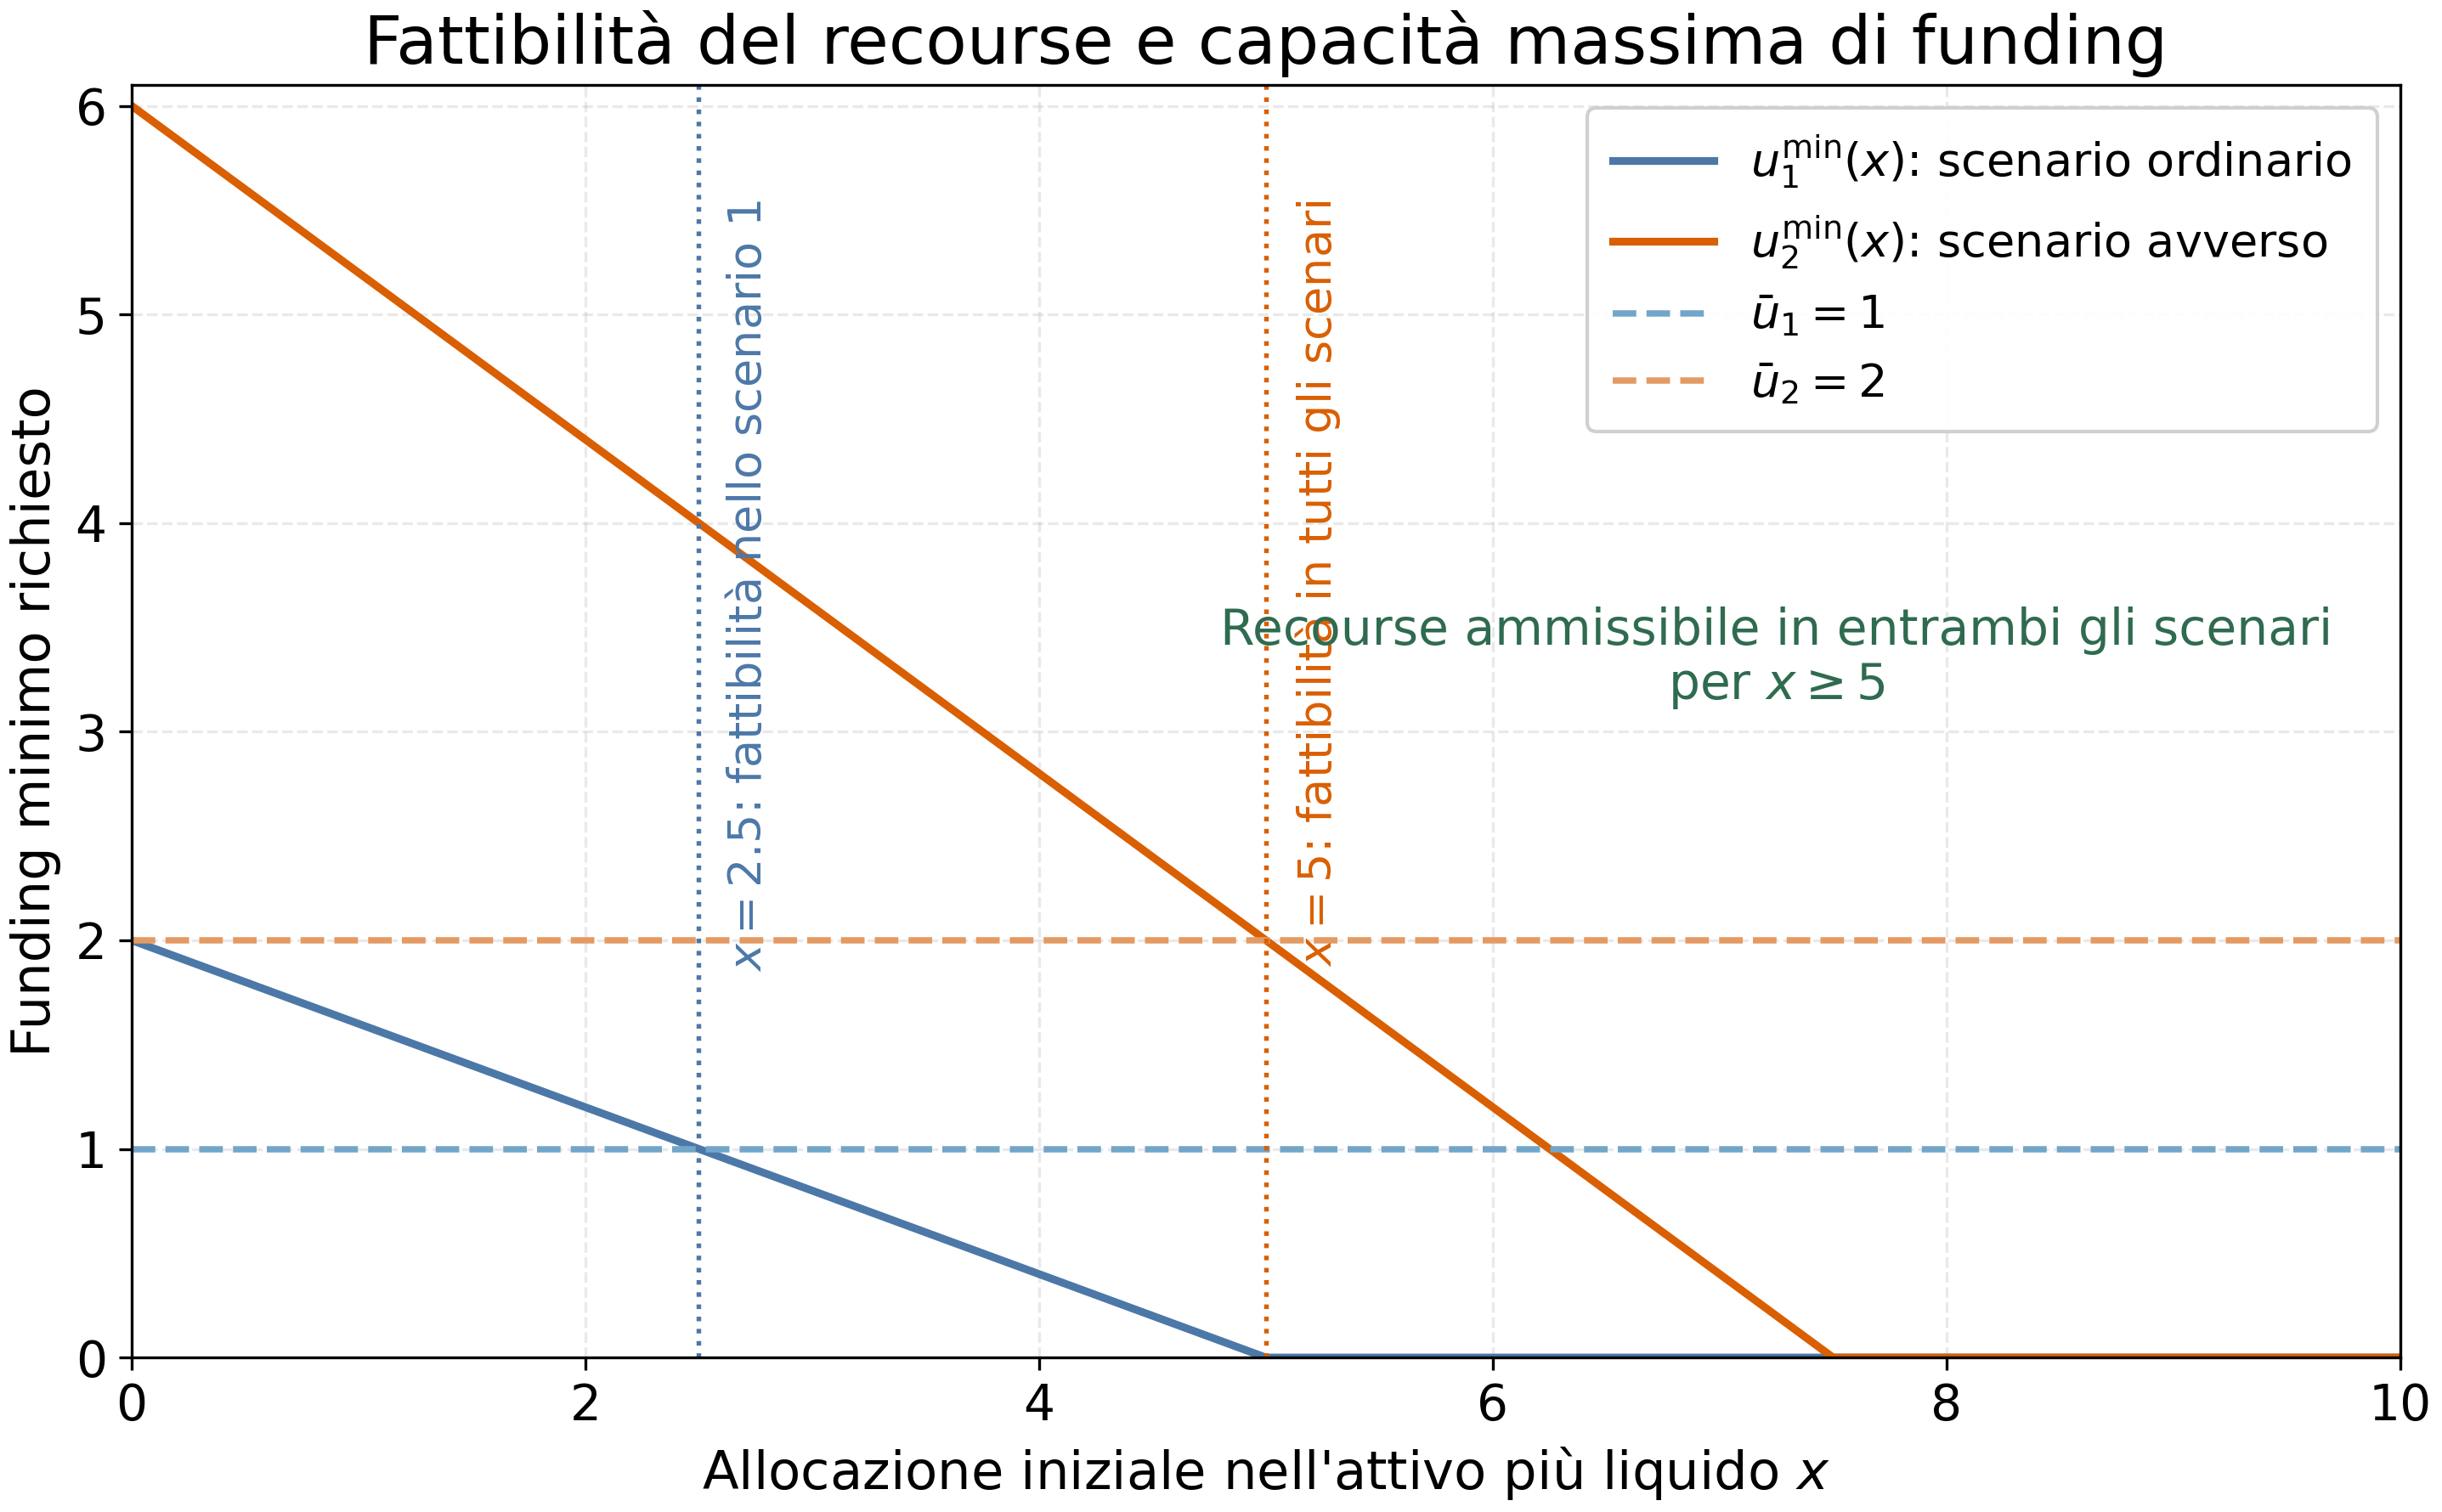
\includegraphics[width=0.94\textwidth]
{../graphics/Cap15_fattibilita_ricorso.png}
\caption{Funding minimo richiesto nei due scenari al variare
dell'allocazione iniziale nella classe di attivo pi\`u liquida.
L'intersezione tra $u_s^{\min}(x)$ e la corrispondente capacit\`a massima
$\bar u_s$ individua la soglia oltre la quale il ricorso diventa ammissibile
nello scenario. Per $x\geq5$ il problema di secondo stadio \`e ammissibile in
entrambi gli scenari.}
\label{fig:cap15-fattibilita-ricorso}
\end{figure}

La figura evidenzia tre regioni. Per

\[
0\leq x<2.5,
\]

la capacit\`a di funding non \`e sufficiente nemmeno nello scenario ordinario.
Per

\[
2.5\leq x<5,
\]

il ricorso \`e ammissibile nello scenario ordinario ma non nello scenario
avverso. Infine, per

\[
x\geq5,
\]

entrambi i problemi di secondo stadio risultano ammissibili.

L'esempio permette ora di distinguere chiaramente la fattibilit\`a del singolo
ricorso dalla propriet\`a di ricorso relativamente completo.

Se l'insieme ammissibile di primo stadio \`e

\[
\mathcal X=[0,10],
\]

il modello non possiede ricorso relativamente completo. Esistono infatti
decisioni ammissibili di primo stadio, come $x=4$, per le quali almeno uno
scenario genera un problema di secondo stadio non ammissibile.

Se invece ulteriori vincoli di primo stadio restringono l'insieme a

\[
\mathcal X=[5,10],
\]

allora, per ogni $x\in\mathcal X$ e per entrambi gli scenari considerati,
esiste almeno una decisione di secondo stadio ammissibile. Il problema
possiede quindi ricorso relativamente completo.

Ci\`o non implica ricorso completo. Le capacit\`a di funding restano infatti
limitate. Se il termine noto del bilancio di secondo stadio producesse un
deficit sufficientemente elevato, nessuna decisione $u_s\leq\bar u_s$ potrebbe
compensarlo. La struttura di ricorso non \`e quindi in grado di fronteggiare
un termine noto arbitrario.

Nel caso SVB--ALM completo lo stesso meccanismo opera attraverso pi\`u date,
pi\`u classi di attivo e pi\`u limiti di funding. Una composizione iniziale
pu\`o risultare ammissibile al primo stadio ma lasciare la banca incapace di
soddisfare uno dei successivi bilanci di liquidit\`a in uno scenario severo.

La fattibilit\`a costituisce quindi il primo filtro nella valutazione di una
decisione stocastica. Soltanto dopo avere verificato l'esistenza delle
decisioni di ricorso ha senso studiarne il valore economico. La sezione
successiva analizza precisamente come la funzione $Q_s(x)$ varia al variare
della decisione iniziale.